\hypertarget{a-few-last-words...}{%
\section{A Few Last Words...}\label{a-few-last-words...}}

This text aims to survey the subject of robotics. However, that is
complete fantasy. Robotics is a huge field and it is not possible to
really touch on all the different areas, delve into some of them and
keep this text under several thousand pages (and a university course
lasting one semester) as well as keeping your interest. So, we must
compromise. This text will focus more on mobile systems and the
technology to implement them than it will on manipulators (robotic arms
and industrial assembly systems) - but not exclusively.

We will approach the subject from a computer science point of view and
write for a computer science audience. This does not imply that
mechanical or electrical engineers should set this down, just that the
presentation will have a distinctly software orientation. Our coverage
will balance more on higher level systems, machine intelligence,
communications and algorithms with less time towards hardware,
controllers, control systems, mechanics, electrical and materials. In
essence we will see the robot as a type of distributed computing system
but one which is aware of how the input data is gathered (sensory
devices) and how the computational results are used (motors, etc).

As a computer scientist, what do you need to know to get started in
Robotics? The list below provides an overview of the topics we will
touch on.

\begin{itemize}
\tightlist
\item
  Simulation and Mathematics
\item
  Behaviors and Motion
\item
  Mechanics, Kinematics and Controls
\item
  Electronics, Signals and Power
\item
  Embedded Systems and Communications
\item
  Distributed Systems
\item
  Sensing, Vision and Ranging
\item
  Planning, Routing, Localization and Navigation
\item
  Mathematics
\end{itemize}

So, we begin our course in mobile robotics fundamentals. Robotics
combines mechanical, electrical and software systems and some of these
systems you need to understand as they fundamentally impact each other.
The goal of this course is to develop sufficient background and
understanding in the subject of mobile autonomous robotics so that you
may become involved with a very dynamic growing industry. As Murphy's
text will indicate, we will break the subject down into three aspects:
perception or sensing, cognition or planning, navigation, localization,
object recognition, and actuation or motion. Perception, cognition and
actuation (sense, plan, act) is a basic theme for this course. However,
there is a bit of the ``chicken and egg'' problem. The subjects are tied
together. Each one can affect the other. It does not make sense to march
entirely through planning, then through sensing and finish with
actuation, no more than it would make sense to give you all of the lines
of one actor in a play, followed by the next actor, and so forth.

The development of the subject has been a bit of a conversation between
engineers and nature. Writing this book in complete historical accuracy
is an interesting idea, but I bet it would become tedious after a couple
of chapters. Our approach here is to give you a taste of a concept and
put it into practice; then relate it to other concepts. Later we return
and go into more detail, put that into practice and relate it to more
involved concepts. This process will cycle through the sense, plan, act
aspects - just as a real robotic system would. In short, I am applying
Agile development to you. You are being 'rapid prototyped' into a
roboticist.

\hypertarget{supplementary-reading}{%
\subsection{Supplementary Reading}\label{supplementary-reading}}

There are many very good books on robotics. The field is well served by
individuals who want to share their knowledge at many different levels
and viewpoints. The important differences are the goals of the books.
Some texts will focus on presenting the mathematics of articulated
manipulators. Some will want to focus on mobile robot path planning.
Others will want to talk about robot controllers using biological
models. All of these points of view are important.

Below is a list of some texts with a brief description on the focus and
audience:

\begin{itemize}
\item
  \begin{description}
  \item[\emph{Principles of Robot Motion}, Choset et al. - This is a
  great book that focuses on the algorithms behind autonomy.]
  It presents a more theoretical treatment of mobile systems and does
  not spend much time on the classic kinematic tools like the D-H
  formalism. For most schools, this would be a graduate level text based
  on the mathematics used in the book although this could be used as an
  elective in a senior course if topics were carefully chosen.
  \texttt{Choset:2005:PRM}
  \end{description}
\item
  \begin{description}
  \item[\emph{Autonomous Mobile Robots}, Siegwart \& Nourbakhsh - This
  is a good shorter book which restricts itself to exactly what the]
  title implies. As indicated in the Preface, the text you are reading
  follows the outline setout by Siegwart \& Nourbakhsh and both are
  heavily influenced by Choset's text. The material on wheels and the
  associated kinematics is more in depth than other subjects in the
  text. Vision, Navigation, Localization and Mapping are briefly touched
  upon but supplementary material is probably warranted.
  \texttt{Siegwart:2004:IAM}
  \end{description}
\item
  \begin{description}
  \item[\emph{Computational Principles of Mobile Robotics}, Dudek \&
  Jenkin - This text is similar in topics and level to Autonomous Mobile
  Robots.]
  Selection between the two would be based on specific topics of
  interest. \texttt{Dudek:2000:CPM}
  \end{description}
\item
  \begin{description}
  \item[\emph{Embedded Robotics}, Braunl - Braunl's book surveys the
  field at a level that a junior in most]
  engineering programs could easily understand. It has a wealth of
  information based on the author's personal experiences. It describes
  many projects and systems at a high level but does not delve deeply
  into the topics. If the hardware discussed in the text were more
  mainstream or current (Arduino, Raspberry Pi, etc), it would make the
  text much more approachable. \texttt{Braunl:2006:ERM}
  \end{description}
\item
  \begin{description}
  \item[\emph{Introduction to Robotics, Analysis, Control,
  Applications}, Niku - Niku's text is a great text for the more
  mechanical side of robotics.]
  There is a wealth of material on kinematic models, inverse kinematics,
  and control. There are well done examples for basic kinematics as
  well. \texttt{niku2010introduction}
  \end{description}
\end{itemize}

The cultural attitudes are strongly affected by books and film:

\begin{figure}
\centering
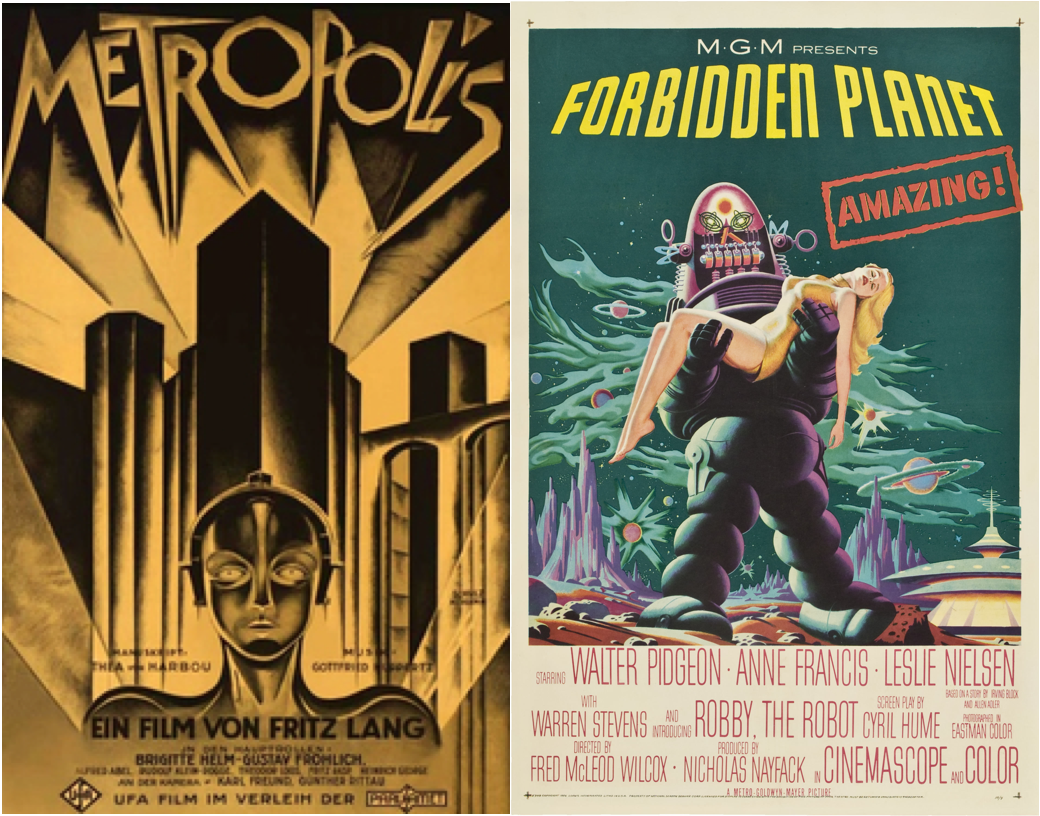
\includegraphics[width=0.85\textwidth,height=\textheight]{IntroductionFigures/poster1.png}
\caption{}
\end{figure}
